\chapter{社区讨论情感对开发者活动的影响}
%%====================================================================

\section{研究背景与问题}

开源社区既是代码协作的技术平台，也是开发者共享知识、讨论问题、交流情感的社会空间。
比特币等加密货币开源项目的讨论区（Issue 区）每天产生大量评论，内容涉及技术问题、协议设计及安全漏洞等议题。
这些评论在传递技术信息的同时承载着丰富的情感色彩——对突破性提案的兴奋与认可、对安全漏洞的焦虑与警觉、代码审查争议中的摩擦与压力，情感极性随项目进展而持续波动。

近年来，情感分析方法被广泛用于考察在线社区中的开发者行为，
已有研究揭示了情感与社区健康、成员流失等现象间的关联
\cite{yang2021differential,fang2009understanding}。
早期工作以问卷调查为主，探讨开发者主观情感体验与参与动机的关系
\cite{shah2006motivation}，发现享受编程本身、声誉积累等内在动机构成开源参与的重要驱动力。
随着自然语言处理技术日趋成熟，基于文本的情感分析逐步取代问卷测量，
成为大规模在线社区情感动态研究的主流方法\cite{guzzi2013}。
Schroter 等人（2010）针对 Bug 报告的研究表明，
报告中的信息质量（如堆栈跟踪）直接影响缺陷修复效率\cite{schroter2010}；
Guzzi 等人则分析了开源软件邮件列表中情感语调与协作效率之间的关系\cite{guzzi2013}。

然而，既有文献大多聚焦于情感对社区参与意愿或成员留存等静态指标的截面影响，
鲜有研究从动态时间序列视角考察情感极性变化如何在短期内左右开发者的具体行为产出，
尤其是代码活动与讨论参与这两类性质迥异的活动形式。
在比特币等加密货币开源项目中，社区情感波动还与外部市场行情高度耦合。
币价大幅上涨往往伴随社区讨论的高涨，技术争议（如区块大小之争）
则可能引发社区内部持续的负面情感聚集\cite{kobayakawa2020impact}。
Bagh 等人（2025）运用 VAR 和格兰杰因果方法分析投资者情感与加密货币市场动态的关系，
发现情感冲击经由社交媒体渠道对市场参与行为产生显著的短期影响\cite{bagh2025investor}。
Kulakowski 和 Frasincar（2023）则专门开发了面向加密货币社区社交媒体文本的
情感分类方法，揭示了该领域文本情感表达的独特模式\cite{kulakowski2023sentiment}。
这种特殊的信息环境使比特币社区成为研究情感动态影响开发者行为的理想场域：
一方面，情感波动幅度大、可观测性强；
另一方面，项目级社区情感（而非个体情感）的测量更易规避问卷方法的主观偏误。

此外，当社区整体情感偏向负面时（如某一安全漏洞被曝光或关键提案遭否决），
开发者面临多重响应选项——提交代码补丁以直接应对问题，
或通过讨论区的评论互动寻求共识、释放压力，抑或两者并行。
这两类活动之间是否存在内生的动态权衡（即加大代码投入后是否相应减少讨论参与），
在既有文献中尚未获得系统性检验。

基于上述研究空白，本章聚焦以下三个问题：
第一，社区讨论情感极性的变化是否在统计意义上“格兰杰引起”（Granger-cause）
后续的开发活动与讨论活动？
第二，情感信号经由何种认知机制作用于开发者的行为决策？
第三，开发活动与讨论活动之间是否存在可观测的跨期替代效应？

对这些问题的回答，一方面有助于从信息行为视角深化对开源开发者激励机制的理解，
另一方面可为开源基金会和社区管理者借助情感信号优化社区治理提供实践依据。


\section{理论假设}

\subsection{情感即信息理论与开发者行为}

本章的核心理论基础为情感即信息理论（Affect-as-Information Theory）
\cite{schwarz1983moods}。
该理论指出，个体在认知判断和行动决策中不仅依赖客观信息，还会将当前情感状态
作为启发性信号加以利用——“我感觉怎么样”（How do I feel?）被转化为
“情况怎么样”（How is it going?）的判断依据。
实验室环境之外，该原理同样适用于在线社区：
当社区整体情感偏向负面时，参与者倾向于将集体情绪解读为“项目存在值得关注的问题”，
从而激发更高的参与意愿。

在比特币开源社区中，Issue 讨论区的情感极性可视为社区健康状况的集体“温度计”。
当社区情感偏向负面——无论是严重 Bug 被发现、关键合并请求引发争议，
还是重大提案受阻——该信号会扩散至整个开发者网络，
提示当前存在需集体应对的技术或社会问题。
Schwarz 和 Clore \citeyear{schwarz1983moods}的原始实验已表明，
即便与判断任务无关的情感（如天气好坏引发的心情）也会影响个体对生活满意度的评价，
可见情感的信息性作用具有相当的普适性，并不局限于实验室情境。

在技术社区语境下，负面情感信号的激励机制可从以下路径加以理解。
其一，集体负面情感意味着现有解决方案尚不令人满意，
这种“不满足”状态激活个体对“行动必要性”的感知，
提高了参与活动的倾向性。
其二，负面情感降低了“当前状态已足够好”的满意度基准，
使开发者对自身活动的边际价值评估更高，参与门槛相应降低。
其三，社区情感信号具有一定的从众效应：
若多数成员表达了对某一问题的担忧，
未参与者更可能将该问题解读为值得关注的重要事项，
从而积极参与其中\cite{yang2021differential}。

根据情感即信息理论，负面情感信号促使开发者从“例行维护”状态切换至“问题解决”模式，
进而增加代码提交、代码审查等具体技术性活动。
需要强调的是，该激励效应的实现并不依赖开发者的自我归因，
而是经由情感的启发式信息功能自动发生——
开发者未必意识到自己在“响应集体情感信号”，
但集体负面情感所传递的问题严峻性感知已足以驱动行为改变。

由此，本章提出假设：

H4：社区讨论情感极性的降低（即负面情感增加），
正向影响开发活动水平。

相应地，负面情感信号不仅激励代码层面的应对，也可激励讨论层面的参与。
社区情绪偏向负面时，开发者同样倾向于通过讨论渠道更积极地表达意见、提出问题或寻求协助，
讨论活动因此也会增加。
在开源社区中，讨论活动（如在 Issue 区发表评论、提出反馈）往往构成代码活动的前置步骤，
也是凝聚共识、协商解决方案的必要过程\cite{guzzi2013}。
负面情感信号所传达的问题紧迫性，同等程度地激活代码层面和讨论层面的行动意愿，
两者皆为响应社区问题的有效手段。

H5：社区讨论情感极性的降低，
正向影响讨论活动水平。

\subsection{目标手段替代理论与活动间替代效应}

在假设 H4 与 H5 的基础上，一个值得追问的后续问题是：
开发活动的增加是否会反过来抑制讨论活动？

目标手段替代理论（Goal-Means Substitution Theory）\cite{kruglanski2002theory}
为此提供了有力的解释框架。
该理论主张，当多种手段可服务于同一目标时，个体对某一手段的使用会降低对其他手段的需求，
亦即不同手段之间存在“认知可替代性”。
在开源社区中，“维护项目健康”是开发者的共同目标，
开发活动（提交代码解决技术问题）与讨论活动（在讨论区交流协商）均为实现该目标的手段。
Kruglanski 等人\citeyear{kruglanski2002theory}指出，
当多个手段在认知上被视为等价或高度重叠时，
使用其中一种会降低使用其他手段的动机，
此即“手段替代”效应。
该理论已在消费行为、利他行为和政治参与等领域获得广泛实证支持。

就开源社区的具体情境而言，当一名开发者在某一特定周大量提交代码以应对社区问题时，
其认知上会完成“问题正在被解决”的任务状态更新，
该更新降低了继续通过讨论来表达关切的驱动力——
代码本身已构成更直接的“行动”表达。
从信号传递的角度看，活跃的代码提交行为也向整个社区传递了“有人在处理问题”的信号，
这在一定程度上降低了其他社区成员参与讨论的感知必要性，
从而在社区层面产生“开发活动→讨论活动减少”的聚合效应。

当开发者已通过加大代码投入来响应问题时，其对进一步参与讨论的边际必要性评估会降低，
后续时期的讨论活动因而减少。

值得注意的是，这种替代效应在时间上存在滞后性。
开发活动对讨论需求的抑制并非即时发生，
而需要一定时间让社区成员感知到代码层面已有积极进展，
讨论的紧迫性方才降低。
这与 GitHub 标准工作流的运转周期相吻合：代码提交后须经过审查与合并，
技术问题被实质性推进之后，相关讨论的紧迫性才随之消退，
故预期替代效应的发生存在一定滞后期。

由此提出：

H6：开发活动水平的增加负向影响后续的讨论活动水平。

三个假设共同构成本章的情感传导机制模型，如图~\ref{fig:path-model-2} 所示：

\begin{figure}[htbp]
    \centering
    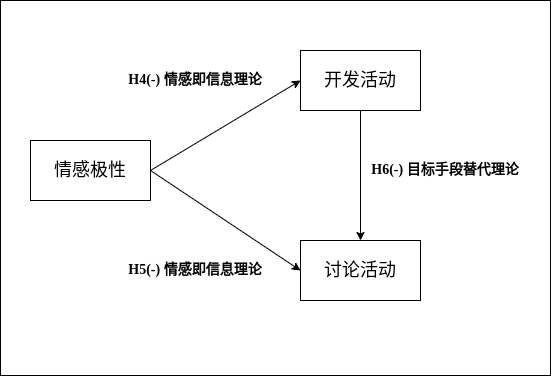
\includegraphics[width=0.58\textwidth]{figures/research_model_2.png}
    \caption{研究二理论假设模型}
    \label{fig:path-model-2}
\end{figure}

\textit{注：箭头方向表示格兰杰因果方向；“$-$”号表示情感极性下降（负面情感增加）
对目标变量的正向效应，或开发活动增加对讨论活动的抑制效应；
具体滞后期数由格兰杰因果检验结合信息准则共同确定，为额外实证发现。}

H4 与 H5 均以情感即信息理论为基础，
共同刻画负面情感信号对两类开发者活动的短期激励效应；
H6 则以目标手段替代理论为基础，描述开发活动对讨论活动的跨期替代效应，
揭示“情感→代码/讨论→讨论”这一多步传导链条。


\section{数据与变量}

\subsection{数据来源}

本研究沿用第四章的比特币开源项目数据框架，
以 GitHub 上的 Bitcoin Core 仓库（\texttt{bitcoin/bitcoin}）为研究对象，
数据来源包括 GitHub Archive（GH Archive）公开数据集与 GitHub REST API。

情感分析所依赖的原始文本数据来源于比特币项目 Issue 区的全量评论，
涵盖2020年1月至2023年12月期间全部 IssueCommentEvent 类型事件。
评论按周聚合后，由大型语言模型对每周文本进行一次性整体评分，
直接生成每周社区情感极性的代理指标。

开发者活动数据同样来源于 GH Archive，
开发活动（$\text{Development}_t$）定义为同一时期的
PushEvent（PE）、CreateEvent（CE）、DeleteEvent（DE）、CommitCommentEvent（CCE）、PullRequestEvent（PRE）与 PullRequestReviewEvent（PRRE）之和，
讨论活动（$\text{Discussion}_t$）定义为同一时期的
IssueCommentEvent（ICE）、IssuesEvent（ISE）与 PullRequestReviewCommentEvent（PRRCE）之和，
两类变量均以周为单位进行统计。

市场控制变量方面，比特币周收益率（$\text{BitcoinReturn}_t$）由 CoinMarketCap 历史价格数据计算得出，
捐赠金额（$\text{DonationAmount}_t$）与受资助人数（$\text{GranteeNumber}_t$）的构建方式与第四章一致，
用以排除外生经济激励对开发者活动的直接干扰。

最终，研究二数据集包含 209 个有效周度观测值，
时间跨度为 2020 年第 1 周至 2023 年第 52 周，
样本期内共观测到 5,000,000 美元以内的多次社区捐赠事件及 4 次授权拨款事件。

样本期的选择基于以下考量。
2020 年初为 Brink 基金会成立的时间节点，
亦是比特币开源社区职业化资助体系逐步建立的起点；
以此作为样本期起点，使研究二与研究一在数据基础上高度重叠，
两项研究共同覆盖的核心时段（2020--2023 年）确保跨研究比较的一致性。
以 2023 年底为终点，系数据获取截止时间的客观限制，
同时确保了样本期涵盖 Brink 多轮定向拨款事件与多次重要的社区技术讨论周期，
为 VAR 模型提供足够数量的时序观测（N=209 周，约 4 年）以保证估计稳定性。
该时段恰好覆盖比特币价格的两轮牛熊周期
（2020--2021 年上行、2022 年下行、2023 年复苏），
比特币收益率变量（$\text{BitcoinReturn}_t$）得以有效控制市场行情对社区情感和活动水平的混淆影响。

数据清洗方面，本研究对以下情况作了处理：
第一，情感评分中的空值周（即当周无任何 Issue 评论）以样本均值填充，
此情况在样本期内极少出现（仅 2 周）；
第二，开发活动和讨论活动中的极端值（超出均值三个标准差的观测），
经 Winsorization（缩尾处理）限定在 99 百分位数，
以降低个别异常高活动周对 VAR 系数估计的杠杆效应；
第三，涉及重大技术会议（如 Bitcoin Core 开发者大会）或 GitHub 平台宕机的周，
通过哑变量加以控制，减少事件性扰动对时间序列估计的影响。

\subsection{情感测量方法}

本研究以大型语言模型（Large Language Model, LLM）为主要工具，对 Issue 评论文本进行情感分析。
相较于基于词典的传统方法（如 VADER\footnote{VADER（Valence Aware Dictionary and sEntiment Reasoner）是一种针对社交媒体文本设计的基于规则的情感分析工具，项目地址：\url{https://github.com/cjhutto/vaderSentiment}。}）和早期预训练模型，
LLM 具备深层语境理解能力，能够识别双关、讽刺、
条件句等复杂语言现象中隐含的情感倾向，
并可借助结构化提示（Prompt）对特定情感维度实施精细化测量
\cite{gilardi2023chatgpt}。
近年研究表明，以 GPT 系列为代表的 LLM 在文本标注任务上的表现
已达到乃至超越众包人工标注的精度，在软件工程文本情感分析
等技术领域亦优于基于词典的传统工具
\cite{zhang2020sentiment}。

模型选择。
本研究采用 Claude Sonnet 4.5\footnote{Claude Sonnet 4.5 由 Anthropic 公司开发，模型 API 文档：\url{https://docs.anthropic.com}。}（claude-sonnet-4.5）作为主要情感打分模型。
为确保结论对情感测量工具选择不敏感，
稳健性检验中分别以 DeepSeek-V3.2（deepseek-v3.2）和 GPT-5.2（gpt-5.2）
两个替代大型语言模型以及 VADER 传统词典方法，
对同一样本进行独立评分并重新估计 VAR 模型（详见第~\ref{sec:robust-2} 节）。
三个 LLM 分属 Anthropic、DeepSeek、OpenAI 三家公司，架构与训练路线各异，
可最大化跨模型多样性；VADER 作为规则型工具，与 LLM 的语义推理在方法论上存在本质差异。
全部 LLM 均通过 OpenAI 兼容接口调用，
推理温度设置为 0 以保证结果的确定性与可重复性。

评分方案。
针对每条 Issue 评论，本研究设计了结构化提示，
要求模型在九分制量表（1--9，5 为中性，1 为极度负面，9 为极度正面）上
对评论的整体情感极性评分，并附简短的评分依据。
模型输出以 JSON 格式返回，其中情感极性分数（\texttt{sentiment\_polarity}）
为本研究的核心变量。
提示还包含六类基本情感（愤怒、厌恶、恐惧、快乐、悲伤、惊讶）
及“失望（期望失验）”维度的分项评分，
为后续情感类型细化分析提供基础数据。
完整的提示词文本见附录 B。
表~\ref{tab:sentiment-example} 展示了三条代表性 Issue 评论的情感极性评分结果及评分依据。

\begin{table}[htbp]
    \centering
    \caption{情感极性评分示例（Claude Sonnet 4.5）}
    \label{tab:sentiment-example}
    \small
    \begin{tabularx}{\textwidth}{c c >{\raggedright\arraybackslash}X >{\raggedright\arraybackslash}X}
        \toprule
        周起始日期 & 极性 & 评论原文（节选） & 评分依据 \\
        \midrule
        2021-08-09 & 7 &
        I've benchmarked \ldots{} and I'm happy to report that I'm seeing a roughly 9\% speedup along with an 8\% reduction in memory usage. &
        文本包含多处性能提升的积极报告、成功的基准测试结果、协作式问题解决以及感谢表达，负面内容极少。 \\
        \midrule
        2023-12-11 & 4 &
        I just wanted to give feedback that this kind of bit me \ldots{} it took some investigating to see why. \ldots{} I don't really get the logic. &
        文本表达了对技术阻碍、反复失败和软件功能未达预期的不满，但整体维持了专业的协作语气。 \\
        \bottomrule
    \end{tabularx}
    \par\vspace{4pt}
    {\small\textit{注：情感极性取值范围为 1--9，5 为中性基准；评论原文为该周 Issue 评论的代表性节选，评分依据由模型对该周全部评论整体评估后生成。}}
\end{table}

文本预处理。
在情感打分前，对每条评论依次执行以下预处理操作：
（1）过滤纯代码片段（以三个反引号 \texttt{```} 包裹的内容），消除代码噪声；
（2）仅保留包含至少 5 个有效词的评论，剔除过短的无意义内容。

聚合与评分策略。
本研究采用"先聚合、后评分"的策略：将每周经预处理的全部有效 Issue 评论
合并为一个文本块，再由大型语言模型对整周文本一次性评分，
直接输出该周情感极性得分，取值域为 $[1, 9]$，以 5 为中性基准，
高于 5 表示正面情感为主，低于 5 则表示负面情感为主。
之所以选择先聚合后评分而非逐条评分再取均值，出于两方面考虑。
其一，不同评论的信息含量和代表性存在差异，
简单算术均值赋予每条评论等权重，
而大型语言模型的评分过程本身即为黑箱，
逐条评分后再聚合会在模型推理误差之上叠加聚合方法的额外误差，
一次性整体评估可减少误差累积。
其二，样本期内 Issue 评论总量庞大，
逐条评分的 API 调用时间成本与资金成本均显著高于周级聚合评分。
样本期内（2020 年至 2023 年）情感均值约为 5.03，
标准差约为 0.63，整体情感以中性偏正为主，
与技术性讨论社区的情感分布特征相符。

稳健性检验中的替代工具对照。
为检验主要结论对情感测量方法选择不敏感，
稳健性检验中引入了三种替代工具：
（1）DeepSeek-V3.2 和 GPT-5.2 两个替代 LLM，采用与主分析相同的结构化提示和九分制量表；
（2）VADER（Valence Aware Dictionary and sEntiment Reasoner），
一种针对社交媒体语言专项优化的规则型情感分析工具\cite{hutto2014vader}，
已在多项开源社区情感研究中得到广泛使用\cite{yang2021differential}，
其 compound 分数（$-1$ 至 $+1$）直接充当情感极性代理变量。
稳健性检验结果详见第~\ref{sec:robust-2} 节。

\subsection{关键变量定义}

研究二涉及三个内生变量和三个外生控制变量，汇总如表~\ref{tab:variables-2} 所示。

\begin{table}[htbp]
    \centering
    \caption{研究二关键变量定义}
    \label{tab:variables-2}
    \small
    \begin{tabularx}{\textwidth}{p{4.5cm}lX}
        \toprule
        变量名称 & 类型 & 定义与说明 \\
        \midrule
        情感极性（$\text{Sentiment}_t$）
            & 内生变量
            & 第 $t$ 周 Issue 评论情感极性均值；
              基于 LLM 的九分制评分（1=极度负面，5=中性，9=极度正面），
              样本内实际观测范围为 $[3,7]$ \\[4pt]
        开发活动（$\text{Development}_t$）
            & 内生变量
            & 第 $t$ 周开发活动总数，包含 PE、CE、DE、CCE、PRE、PRRE，
              反映社区整体开发活动强度 \\[4pt]
        讨论活动（$\text{Discussion}_t$）
            & 内生变量
            & 第 $t$ 周讨论活动总数，包含 ICE、ISE、PRRCE，
              反映社区整体讨论参与强度 \\[4pt]
        比特币收益率（$\text{BitcoinReturn}_t$）
            & 外生控制
            & 第 $t$ 周比特币价格收益率，控制加密货币市场行情波动 \\[4pt]
        捐赠金额（$\text{DonationAmount}_t$）
            & 外生控制
            & 第 $t$ 周非定向捐款金额（千美元），控制外生资金激励 \\[4pt]
        受资助人数（$\text{GranteeNumber}_t$）
            & 外生控制
            & 第 $t$ 周定向资助受益人数量，控制定向激励效应 \\
        \bottomrule
    \end{tabularx}
\end{table}

\subsection{描述性统计}

表~\ref{tab:desc-stats-2} 报告了研究二主要变量的描述性统计信息。

\begin{table}[htbp]
    \centering
    \small
    \caption{研究二变量描述性统计（N=209周）}
    \label{tab:desc-stats-2}
    \begin{tabularx}{\textwidth}{Xrrrrr}
        \toprule
        变量 & 均值 & 标准差 & 最小值 & 最大值 & 观测数 \\
        \midrule
        情感极性（$Sentiment_t$） & 5.026 & 0.628 & 3.000 & 7.000 & 209 \\
        开发活动（$Development_t$）      & 333.47 & 158.24 & 11 & 922 & 209 \\
        讨论活动（$Discussion_t$）   & 604.98 & 242.52 & 53 & 1479 & 209 \\
        比特币收益率（$BitcoinReturn_t$）    & 0.0076 & 0.0876 & $-$0.415 & 0.320 & 209 \\
        捐赠金额（$DonationAmount_t$）  & 42.87 & 369.09 & 0 & 5{,}000 & 209 \\
        受资助人数（$GranteeNumber_t$）     & 0.038 & 0.308 & 0 & 4 & 209 \\
        \bottomrule
    \end{tabularx}
\end{table}

从描述性统计来看，情感极性均值为 5.026，略高于中性值 5，
表明样本期内比特币开源社区整体情感温和正向，
但标准差达 0.628，周间情感波动较为显著。
开发活动均值为 333.47 次/周，标准差 158.24，高变异系数反映了开发者活动的周期性波动；
讨论活动均值 604.98 次/周，约为开发活动的两倍，讨论参与构成开源社区最主要的活动形式。
捐赠金额（$\text{DonationAmount}_t$）标准差极大，反映其非连续性——多数周无捐赠，
少数周出现高额捐赠事件（最大值为 5,000 千美元），这与比特币开源项目的实际融资模式一致。

表~\ref{tab:corr-2} 报告了研究二主要变量的 Pearson 相关系数矩阵。

\begin{table}[htbp]
    \centering
    \caption{研究二主要变量相关系数矩阵}
    \label{tab:corr-2}
    \small
    \begin{tabularx}{\textwidth}{p{3cm}XXXXXX}
        \toprule
         & 情感极性 & 开发活动 & 讨论活动 & 收益率 & 捐赠金额 & 受资助人数 \\
        \midrule
        情感极性     & 1.000 & & & & & \\
        开发活动     & 0.123   & 1.000 & & & & \\
        讨论活动     & 0.127   & 0.522 & 1.000 & & & \\
        收益率       & 0.113   & 0.095 & 0.124 & 1.000 & & \\
        捐赠金额     & 0.136   & 0.015 & $-$0.060 & 0.004 & 1.000 & \\
        受资助人数   & $-$0.030 & 0.054 & 0.009 & $-$0.109 & $-$0.010 & 1.000 \\
        \bottomrule
    \end{tabularx}
    \begin{minipage}{\textwidth}
        \vspace{0.3em}
        \footnotesize 注：N=209。通常认为相关系数绝对值大于 0.6 表示高相关。
        情感极性=$Sentiment_t$；开发活动=$Development_t$；讨论活动=$Discussion_t$；
        收益率=$BitcoinReturn_t$（比特币周收益率）；
        捐赠金额=$DonationAmount_t$（当周非定向捐款金额，千美元）；
        受资助人数=$GranteeNumber_t$（当周定向资助受益人数量）。
    \end{minipage}
\end{table}

就相关系数矩阵而言，所有变量两两间的相关系数绝对值均低于 0.6，
各变量之间不存在高相关关系，多重共线性风险较低，适合纳入同一 VAR 模型。
其中开发活动与讨论活动的相关系数最高（$r = 0.522$），
接近但未超过 0.6 的高相关阈值，表明两类活动在同期截面上有一定协同趋势。
但这并不排除时间序列层面两者存在跨期替代关系：
截面相关捕捉的是同一时点的共同波动（受共同外生冲击驱动），
跨期替代则是开发活动影响后续讨论活动的动态效应，两种关系并不矛盾。
情感极性与开发活动（$r = 0.123$）、讨论活动（$r = 0.127$）的相关系数均较低，
情感与活动在同期截面层面的线性关联较弱。
需指出的是，本研究核心假设（H4、H5）关注的是负面情感对后续活动的滞后激励效应，
与截面相关属于不同的分析维度。
比特币收益率与情感极性的相关系数亦较低（$r = 0.113$），
市场行情并非社区情感的主要同期驱动因素，
有助于排除“牛市→正面情感→活动增减”的混淆路径。
其余变量对间的相关系数均接近于零，进一步确认了变量间的低相关性。


\section{研究方法：向量自回归模型}

\subsection{VAR 模型的选择依据}

情感、开发活动与讨论活动三个核心变量间存在理论上的双向动态反馈关系：
情感影响后续活动，活动反过来也可能塑造社区情感氛围。
在该系统中，任何单方程回归模型（如普通最小二乘法或固定效应面板模型）
均面临内生性问题——若对情感变量进行单独回归，开发活动和讨论活动对情感的反向影响
将导致估计量有偏。

向量自回归（Vector Autoregression, VAR）模型由 Sims（1980）\cite{sims1980macroeconomics}提出，
将所有变量均设为内生变量，同时以其自身及系统中其他变量的若干滞后期为预测量，
在同一框架内对多变量时间序列系统进行无约束估计。
VAR 模型具有三方面优势：
第一，无需对变量因果方向作先验假设，适合探索性分析；
第二，可通过格兰杰因果检验\cite{granger1969investigating}在统计意义上识别变量间的预测关系；
第三，脉冲响应函数（IRF）和方差分解（FEVD）
能够对动态效应的规模与持续时间加以可视化和量化，
是时间序列因果分析的标准工具。

\subsection{模型设定}

设三元内生变量向量
$\mathbf{y}_t = [\text{Sentiment}_t,\ \text{Development}_t,\ \text{Discussion}_t]'$，
外生控制变量向量
$\mathbf{x}_t = [\text{BitcoinReturn}_t,\ \text{DonationAmount}_t,\ \text{GranteeNumber}_t]'$，
则含外生变量的 VAR($p$) 模型为：

\begin{equation}
\label{eq:var-model}
\mathbf{y}_t = \mathbf{c} + \sum_{k=1}^{p} \mathbf{A}_k \mathbf{y}_{t-k}
+ \mathbf{B} \mathbf{x}_t + \boldsymbol{\varepsilon}_t
\end{equation}

其中 $\mathbf{c}$ 为截距向量，$\mathbf{A}_k$（$k=1,\ldots,p$）为各滞后期的系数矩阵，
$\mathbf{B}$ 为外生变量系数矩阵，
$\boldsymbol{\varepsilon}_t \sim \text{i.i.d.} \mathcal{N}(\mathbf{0}, \boldsymbol{\Sigma})$
为误差项向量。

\subsection{分析流程}

本章按以下六步开展实证分析：

第一步，平稳性检验。
对三个内生变量分别进行增广迪基-富勒（Augmented Dickey-Fuller, ADF）单位根检验，
确认序列平稳性，以满足 VAR 水平模型估计的基本前提。
若变量为非平稳序列（I(1)），则需进行差分处理或引入协整分析框架（VECM 模型）；
若变量为平稳序列（I(0)），则可直接在水平值上估计 VAR 模型。

第二步，最优滞后阶数选择。
基于赤池信息准则（AIC）与贝叶斯信息准则（BIC/SBIC）
确定最优滞后阶数 $p$，在拟合优度与参数简约性之间取得平衡。
AIC 偏向选择较高的滞后阶数以保留更多动态信息，
BIC 对参数数量惩罚更重，倾向于更简约的模型。
两者建议不一致时，综合考量 AIC 在动态预测场景下对欠拟合的适度容忍性进行取舍。

第三步，VAR($p$) 模型估计。
以最优滞后阶数估计含外生变量的 VAR($p$) 模型，
采用小样本自由度修正（Degree of Freedom Correction, DFK 修正）提高估计稳健性。
DFK 修正通过用自由度调整的协方差矩阵替代最大似然估计的协方差矩阵，
在小样本下相较于标准 VAR 估计具有更好的有限样本性质。

第四步，格兰杰因果检验。
对各方程进行格兰杰因果沃尔德检验（Granger Causality Wald Test），
通过 $\chi^2$ 统计量在 0.05 的显著性水平下判断变量间的格兰杰因果关系，
直接对应 H4（Sentiment Granger-causes Development）、
H5（Sentiment Granger-causes Discussion）和 H6（Development Granger-causes Discussion）的检验。
反向检验（Development/Discussion Granger-causes Sentiment）则用于验证情感变量的外生性。

第五步，脉冲响应函数（IRF）分析。
构建 $3 \times 3$ 的脉冲响应函数矩阵，以可视化单变量冲击的系统动态效应。
采用乔列斯基（Cholesky）正交分解对新息协方差矩阵加以识别，
变量排序设定为 Sentiment → Development → Discussion。
排序依据如下：情感作为社会信号先于行为输出发生（认知先于行动），
而开发活动的周转时间通常短于讨论活动（提交代码的决策较快，参与讨论的决策较慢）。
以 bootstrapping 方法估计 95\% 置信区间，追踪 10 期（约 10 周）的脉冲响应路径。

第六步，预测误差方差分解（FEVD）。
量化情感冲击对开发活动和讨论活动预测误差方差的解释占比，
评估情感信号在整个系统中的相对重要性。
FEVD 将 $h$ 步预测误差方差分解为各变量正交冲击的解释份额，
反映各变量对系统波动的解释能力，是对格兰杰因果检验和 IRF 分析的有益补充。


\section{实证结果}

\subsection{平稳性检验}

在估计 VAR 模型之前，对三个内生变量分别进行增广迪基-富勒（ADF）单位根检验，
检验形式包含截距项，滞后阶数依据 AIC 准则自动选择。
表~\ref{tab:adf-test} 报告了平稳性检验结果。

\begin{table}[htbp]
    \centering
    \small
    \caption{ADF 单位根检验结果}
    \label{tab:adf-test}
    \begin{tabularx}{\textwidth}{Xrrrp{3cm}}
        \toprule
        变量 & ADF 统计量 & 滞后阶数 & 1\% 临界值 & 结论 \\
        \midrule
        情感极性（$Sentiment_t$） & $-$15.379 & 0 & $-$3.474 & 平稳 (I(0))*** \\
        开发活动（$Development_t$）      & $-$5.352  & 0 & $-$3.474 & 平稳 (I(0))*** \\
        讨论活动（$Discussion_t$）   & $-$5.935  & 0 & $-$3.474 & 平稳 (I(0))*** \\
        比特币收益率（$BitcoinReturn_t$）    & $-$13.029 & 0 & $-$3.474 & 平稳 (I(0))*** \\
        捐赠金额（$DonationAmount_t$）  & $-$14.010 & 0 & $-$3.474 & 平稳 (I(0))*** \\
        受资助人数（$GranteeNumber_t$）     & $-$14.579 & 0 & $-$3.474 & 平稳 (I(0))*** \\
        \bottomrule
    \end{tabularx}
    \begin{minipage}{\textwidth}
        \vspace{0.3em}
        \footnotesize 注：检验形式含截距，滞后阶数为 0；
        *** 表示在 1\% 显著性水平下拒绝单位根假设（序列平稳）；
        1\% 临界值约为 $-3.474$（MacKinnon，样本量 $N = 208$）。
        BitcoinReturn、DonationAmount、GranteeNumber 为外生控制变量，同步通过 ADF 检验。
    \end{minipage}
\end{table}

六个序列的 ADF 统计量均远小于 1\% 显著性水平下的临界值，
三个内生变量（情感极性、开发活动和讨论活动）
及三个外生控制变量（BitcoinReturn、DonationAmount、GranteeNumber）均为零阶单整序列（I(0)），
原始序列本身已满足平稳性要求，无需一阶差分处理。
该结果为后续 VAR 水平模型的直接估计奠定了前提，
变量间的长期关系可在水平形式下直接检验，
无需额外引入协整分析框架。

\subsection{最优滞后阶数}

表~\ref{tab:lag-selection} 报告了基于 AIC、HQIC 和 SBIC 准则的滞后阶数选择结果。

\begin{table}[htbp]
    \centering
    \caption{VAR 模型最优滞后阶数选择}
    \label{tab:lag-selection}
    \begin{tabularx}{\textwidth}{cXrrrr}
        \toprule
        滞后阶数 & 对数似然值 & LR 统计量 & FPE & AIC & SBIC \\
        \midrule
        0 & $-$2829.39 & --- & 3.8e+08 & 28.273 & 28.470 \\
        1 & $-$2586.23 & 486.32*** & 3.7e+07 & 25.943 & 26.288* \\
        2 & $-$2566.63 & 39.19*** & 3.3e+07* & 25.837* & 26.330 \\
        3 & $-$2559.75 & 13.77 & 3.4e+07 & 25.858 & 26.499 \\
        4 & $-$2556.65 & 6.19 & 3.6e+07 & 25.917 & 26.706 \\
        \bottomrule
    \end{tabularx}
    \begin{minipage}{\textwidth}
        \vspace{0.3em}
        \footnotesize 注：*表示该准则下的最优滞后阶数；样本量 N=201（滞后8期时）。
              AIC 在滞后2期取最优值 25.8372；SBIC 在滞后1期取最优值。
    \end{minipage}
\end{table}

AIC 准则建议选择滞后 2 期（AIC = 25.8372），
SBIC 准则建议选择滞后 1 期（SBIC = 26.2877），
二者产生分歧。AIC 对欠拟合（under-fitting）的惩罚较弱，
在动态预测场景中更适合保留充分的滞后期信息；
SBIC 在小样本下倾向于过度惩罚模型复杂度，
所选单期模型可能遗漏重要的动态效应。
综合上述考量，本研究选定 AIC 建议的 VAR(2) 作为基准模型。

\subsection{VAR 模型回归结果}

表~\ref{tab:var-results} 报告了 VAR(2) 模型各方程中关键系数的估计结果。

\begin{table}[htbp]
    \centering
    \caption{VAR(2) 模型回归结果（核心系数）}
    \label{tab:var-results}
    \small
    \begin{tabularx}{\textwidth}{p{3.2cm}p{3.2cm}XXXX}
        \toprule
        因变量 & 预测变量 & 系数 & 标准误 & $z$ 值 & $p$ 值 \\
        \midrule
        \multicolumn{6}{l}{\textit{开发活动方程（$R^2 = 0.617$，$\chi^2 = 316.67$，$p < 0.001$）}} \\[2pt]
        开发活动$_t$ & 情感极性$_{t-1}$ & $-37.199$ & 11.509 & $-3.23$ & $0.001$*** \\
                 & 情感极性$_{t-2}$ & $-21.711$ & 11.689 & $-1.86$ & $0.063$ \\
                 & 开发活动$_{t-1}$      & $0.853$   & 0.119  & $7.17$  & $0.000$*** \\
                 & 开发活动$_{t-2}$      & $-0.022$  & 0.119  & $-0.18$ & $0.854$ \\
                 & 讨论活动$_{t-1}$   & $-0.113$  & 0.069  & $-1.63$ & $0.103$ \\
                 & 讨论活动$_{t-2}$   & $0.052$   & 0.069  & $0.76$  & $0.447$ \\[6pt]
        \multicolumn{6}{l}{\textit{讨论活动方程（$R^2 = 0.548$，$\chi^2 = 239.20$，$p < 0.001$）}} \\[2pt]
        讨论活动$_t$ & 情感极性$_{t-1}$ & $-61.230$ & 19.369 & $-3.16$ & $0.002$*** \\
                    & 情感极性$_{t-2}$ & $-27.353$ & 19.672 & $-1.39$ & $0.164$ \\
                    & 开发活动$_{t-1}$      & $0.341$   & 0.200  & $1.71$  & $0.088$ \\
                    & 开发活动$_{t-2}$      & $-0.516$  & 0.200  & $-2.58$ & $0.010$** \\
                    & 讨论活动$_{t-1}$   & $0.433$   & 0.116  & $3.73$  & $0.000$*** \\
                    & 讨论活动$_{t-2}$   & $0.379$   & 0.116  & $3.27$  & $0.001$*** \\[6pt]
        \multicolumn{6}{l}{\textit{情感极性方程（$R^2 = 0.076$，$\chi^2 = 16.20$，$p = 0.063$）}} \\[2pt]
        情感极性$_t$ & 情感极性$_{t-1}$ & $-0.053$ & 0.071 & $-0.75$ & $0.453$ \\
                      & 开发活动$_{t-1}$      & $9.41\times10^{-6}$ & 0.001 & $0.01$ & $0.990$ \\
                      & 讨论活动$_{t-1}$   & $-0.001$ & 0.000 & $-1.23$ & $0.218$ \\
        \bottomrule
    \end{tabularx}
    \begin{minipage}{\textwidth}
        \vspace{0.3em}
        \footnotesize 注：*** $p < 0.01$，** $p < 0.05$，* $p < 0.1$；
              情感极性=$Sentiment_t$，开发活动=$Development_t$，讨论活动=$Discussion_t$。
              所有方程均加入比特币收益率（$BitcoinReturn_t$）、捐赠金额（$DonationAmount_t$）、受资助人数（$GranteeNumber_t$）作为外生控制变量，系数从略。
              样本量 $N = 207$（受滞后期损失）。
    \end{minipage}
\end{table}

就 Development 方程而言，情感极性滞后一期（$Sentiment_{t-1}$）对开发活动的影响系数为
$-37.199$（$z = -3.23$，$p = 0.001$），高度显著。
系数为负意味着情感极性下降一个单位（即情感偏向负面），
后续一周的开发活动增加约 37 次，与 H4 的预测方向一致。
开发活动自身一期滞后（$Development_{t-1}$）系数为 0.853，表明开发活动具有显著的自身惯性，
前一周的活动水平对当期有强预测力。

就 Discussion 方程而言，情感极性滞后一期（$Sentiment_{t-1}$）的系数为
$-61.230$（$z = -3.16$，$p = 0.002$），同样高度显著。
情感下降一个单位对应后续一周讨论活动增加约 61 次，H5 获得支持。
值得关注的是，情感对讨论活动的影响系数（绝对值 61.23）明显高于对开发活动的影响系数
（绝对值 37.20），表明开发者在情感驱动下更倾向于通过讨论渠道作出反应。
与此同时，前两期开发活动（$Development_{t-2}$）对讨论活动的系数为
$-0.516$（$z = -2.58$，$p = 0.010$），
即前两期开发活动水平每增加一次，当期讨论活动约减少 0.52 次，H6 获得支持。该结果进一步揭示了替代效应的具体滞后结构为两期（约两周），与 GitHub 工作流的典型周转时间相符。

情感方程（Sentiment 方程）的 $R^2$ 仅为 0.076，联合显著性检验（$p = 0.063$）
恰处于边界水平，开发活动与讨论活动对情感的反向影响较弱。
这与情感作为外生社会信号的理论定位相符——情感主要由社区外部事件（如安全漏洞曝光、
重大提案被否决）所驱动，而非被开发者活动塑造。

关于控制变量，三个外生变量（BitcoinReturn、DonationAmount、GranteeNumber）在 Development 方程和 Discussion 方程
中均未达到 5\% 的统计显著性（系数从略）。该结果具有重要的理论意涵：
在控制情感信号之后，比特币市场收益率、外部捐赠规模和授权拨款数量
对开发活动和讨论活动的边际影响均不显著。
这与第四章的发现形成有意义的对比——在个体层面，捐赠信息披露对部分开发者的活动水平
具有显著的事件驱动效应（尤其是“Brink 定向披露”事件的负面效应）；
而在社区聚合层面，这些外部经济激励被情感信号所主导，
对整体开发者活动的独立预测力相对有限。
此发现提示，在时间序列层面，情感构成开发者行为波动的更核心信息驱动力，
外部物质激励的影响更多体现在个体截面的异质性上，而非社区整体活动的动态变化中。

就模型整体拟合而言，Development 方程 $R^2 = 0.617$，Discussion 方程 $R^2 = 0.548$，
VAR(2) 模型分别解释了开发活动方差的 61.7\% 和讨论活动方差的 54.8\%，
拟合质量可接受。Development 方程联合显著性检验 $\chi^2 = 316.67$（$p < 0.001$），
Discussion 方程 $\chi^2 = 239.20$（$p < 0.001$），均高度显著。

\subsection{格兰杰因果检验}

为在统计意义上进一步检验变量间的动态因果关系，
表~\ref{tab:granger} 报告了基于沃尔德检验（Wald Test）的格兰杰因果检验结果。

\begin{table}[htbp]
    \centering
    \caption{格兰杰因果检验结果}
    \label{tab:granger}
    \begin{tabularx}{\textwidth}{p{3.5cm}Xrrr}
        \toprule
        因变量（方程） & 排除变量 & $\chi^2$ 统计量 & 自由度 & $p$ 值 \\
        \midrule
        开发活动（$Development$）     & 情感极性（$Sentiment$） & 13.967 & 2 & $0.001$*** \\
        开发活动（$Development$）     & 讨论活动（$Discussion$）   & 4.406  & 2 & $0.110$ \\
        讨论活动（$Discussion$）  & 情感极性（$Sentiment$） & 11.979 & 2 & $0.003$*** \\
        讨论活动（$Discussion$）  & 开发活动（$Development$）      & 8.650  & 2 & $0.013$** \\
        情感极性（$Sentiment$） & 开发活动（$Development$）      & 0.330  & 2 & $0.848$ \\
        情感极性（$Sentiment$） & 讨论活动（$Discussion$）   & 2.012  & 2 & $0.366$ \\
        \bottomrule
    \end{tabularx}
    \begin{minipage}{\textwidth}
        \vspace{0.3em}
        \footnotesize 注：*** $p < 0.01$，** $p < 0.05$；“因变量/排除变量”表示
              “排除变量是否格兰杰引起因变量”的检验；自由度 = 滞后阶数 $p = 2$。
    \end{minipage}
\end{table}

格兰杰因果检验结果对三个研究假设构成清晰支持：

其一，情感显著格兰杰引起开发活动（$\chi^2 = 13.967$，$p = 0.001$），
H4 成立——情感极性变化在统计意义上能够预测后续开发活动水平。

其二，情感显著格兰杰引起讨论活动（$\chi^2 = 11.979$，$p = 0.003$），
H5 成立——情感信号对讨论活动同样具有预测能力。

其三，开发活动显著格兰杰引起讨论活动（$\chi^2 = 8.650$，$p = 0.013$），
H6 成立——开发活动的增加确能预测后续讨论活动的下降。

反向检验结果同样值得关注：
开发活动和讨论活动均不格兰杰引起情感变量
（Development → Sentiment：$\chi^2 = 0.330$，$p = 0.848$；
Discussion → Sentiment：$\chi^2 = 2.012$，$p = 0.366$），
进一步印证了情感变量作为外生信号输入而非系统内反馈的角色定位。

从格兰杰因果检验的完整图景看，
系统中存在两条清晰的信息-行为传导路径。
第一条，情感→代码（$p = 0.001$）和情感→讨论（$p = 0.003$），
对应情感即信息理论所描述的“情感信号激活行动”机制。
第二条，代码→讨论（$p = 0.013$），
对应目标手段替代理论所描述的“活动间替代”机制。
两条路径共同构成“情感→\{代码，讨论\}→讨论”的三角传导链条，
开发活动同时作为情感信号的输出端和讨论活动的替代手段，
在整个系统中处于枢纽位置。

另须注意的是，讨论活动对情感的预测效果未达显著水平
（Discussion → Sentiment：$\chi^2 = 2.012$，$p = 0.366$）。
$p$ 值高于 0.05 阈值，讨论活动对情感的潜在影响可以忽略，
由此排除了“大量负面评论导致更多负面评论”的正反馈循环假设——
若存在此种循环，情感即信息效应有可能被放大效应所混淆。
反向格兰杰检验的不显著结果为情感信号的外生性提供了关键支持，
构成本研究因果识别策略的重要一环。

\subsection{脉冲响应分析}

图~\ref{fig:irf-study2} 报告了 VAR(2) 模型的 $3 \times 3$ 脉冲响应函数矩阵，
每幅子图显示某一变量受到一个标准差正向冲击后，
系统中各变量在随后 10 期内的动态响应路径（实线为点估计，阴影为 95\% 置信区间）。

\begin{figure}[htbp]
    \centering
    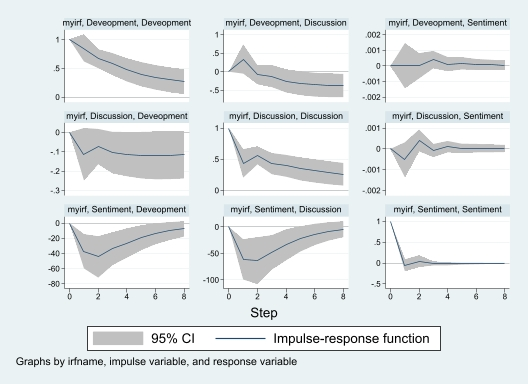
\includegraphics[width=0.92\textwidth]{figures/irf_study2.jpg}
    \caption{VAR(2) 模型脉冲响应函数（$3\times3$ 矩阵）}
    \label{fig:irf-study2}
\end{figure}

\textit{注：行表示施加冲击的变量（第1行 Development、第2行 Discussion、第3行 Sentiment），
列表示被响应变量（第1列 Development、第2列 Discussion、第3列 Sentiment）；
横轴为期数（周），纵轴为响应幅度；
灰色阴影区域为 95\% 置信区间。}

就情感冲击行（第三行）而言，情感正向冲击（即情感极性上升）
对开发活动（第3行第1列）产生负向响应：
开发活动在冲击后第 1--2 期显著下降（响应幅度约 $-60$ 至 $-80$），
随后逐渐回归基线，置信区间在第 1--3 期不包含零。
该响应模式与 H4 方向一致：
情感极性上升（即负面情感减少）导致开发活动减少，
等价于情感极性下降（负面情感增加）触发开发活动增加。

类似地，情感正向冲击对讨论活动（第3行第2列）亦产生负向响应，
且响应幅度更大（约 $-50$ 至 $-100$），
第 1--2 期置信区间不含零，与 H5 方向一致。

开发活动冲击对讨论活动（第1行第2列）的响应在第 1 期为正（短期互补），
第 2 期后转为负向，第 2--3 期置信区间不含零。
这一跨期模式印证了 H6 假设的替代效应，并揭示了其具体时序特征：
开发活动增加后约两周，对讨论活动产生显著抑制。
第 1 期的短暂正向响应可作如下解释：开发活动增加伴随相应的代码审查讨论，
代码被合并之前，讨论活动与开发活动存在短期协同；
而代码一旦合并、问题得到处理、相关 Issue 被关闭，讨论活动才随之下降。
该细节进一步支持了“代码→审查→问题解决→讨论需求消退”的完整传导链条。

情感冲击对情感自身（第3行第3列）的响应在第 1 期为正
（反映冲击本身的即时效应），随即迅速衰减至接近零，
表明情感不具有显著持续性，社区情感波动的自相关特征较弱，
与情感主要由外部事件驱动而非由系统内在动力主导的解释一致。
开发活动自身冲击响应（第1行第1列）呈现 8 期内缓慢衰减的正向响应，
印证了开发活动的强自相关性（滞后一期系数 0.853）；
讨论活动的自身冲击响应（第2行第2列）同样表现出显著持续性，
反映了社区讨论的连续性和话题惯性。

综观 IRF 图的整体模式，第三行（情感冲击）对开发活动和讨论活动的负向响应路径，
以及第一行（开发活动冲击）对讨论活动的跨期负向响应，
构成本研究情感传导机制的可视化核心证据，
与格兰杰因果检验和 VAR 系数估计结果相互印证，
共同形成研究假设 H4、H5、H6 的三角验证体系。

\subsection{预测误差方差分解}

表~\ref{tab:fevd} 报告了 8 步预测的方差分解结果，
量化了情感、开发活动、讨论活动三个变量对各自预测误差方差的相对解释占比。

\begin{table}[htbp]
    \centering
    \caption{预测误差方差分解（步数=8）}
    \label{tab:fevd}
    \begin{tabularx}{\textwidth}{p{3.5cm}XXX}
        \toprule
        被响应变量 & 情感极性解释占比（\%） & 开发活动解释占比（\%） & 讨论活动解释占比（\%） \\
        \midrule
        开发活动（$Development$）    & 4.87 & 91.70 & 3.43 \\
        讨论活动（$Discussion$） & 4.35 & 59.63 & 36.02 \\
        \bottomrule
    \end{tabularx}
    \begin{minipage}{\textwidth}
        \vspace{0.3em}
        \footnotesize 注：步数 = 8 期（8 周）；各行之和约为 100\%。
              基于 Cholesky 正交分解，排序为情感极性（Sentiment）→ 开发活动（Development）→ 讨论活动（Discussion）。
    \end{minipage}
\end{table}

方差分解结果呈现以下规律。

就开发活动的预测方差而言，91.70\% 由开发活动自身解释，
情感解释占比为 4.87\%，讨论活动解释占比为 3.43\%。
开发活动的高度自解释性反映了其强自相关特性（滞后一期系数达 0.853），
也意味着情感对开发活动的影响虽统计显著，但在方差层面相对有限。

就讨论活动的预测方差而言，开发活动解释占比高达 59.63\%，
显著超过讨论活动自身的 36.02\%，情感解释占比为 4.35\%。
开发活动对讨论活动方差的高解释份额进一步印证了 H6 中代码-讨论替代效应的系统性重要性：
开发活动变动是驱动讨论活动波动的主要外因，其重要性甚至超过讨论活动本身的惯性。

两个变量的情感解释比例（约 4--5\%）绝对数值虽不高，
但对应的格兰杰因果效应和 VAR 系数均高度显著，
表明情感的影响更多体现在方向性触发（激活效应）而非幅度上的持续主导。

理解上述方差分解结果，须结合开源开发活动本身的特征。
开发活动的高度自解释性（91.70\%）反映了开发者工作节奏具有较强的个人惯性：
已活跃的开发者倾向于在随后几周保持活跃（“活跃惯性”），
进入低活跃状态的开发者也倾向于在短期内维持低活跃水平。
该特征与开源志愿者的“项目冲刺”工作模式相吻合——
开发者往往在特定时期集中爆发式地大量提交，而后进入相对安静的间歇期。
相比之下，情感信号作为外部信息输入，能在特定时机“打破”这种惯性，
激发超出历史基准的额外活动。

就讨论活动而言，开发活动解释的 59.63\% 方差份额是最具理论意涵的发现。
讨论活动的波动在很大程度上是开发活动波动的“影子”：
开发活动活跃的周，随后的讨论容易出现系统性变化（先增后减）。
该发现直接验证了 H6 所揭示的代码-讨论替代机制的系统性重要性，
表明在社区层面该替代效应为持续稳定的规律性现象，而非个别时期的偶然观测。


\section{稳健性检验}
\label{sec:robust-2}

为验证主要结论的稳健性，本章从六个维度对基准 VAR(2) 结果进行检验。

\subsection{更换情感变量：单独使用负向情感指标}

主分析中的情感极性（Sentiment）是一个综合指标，
同时包含正向和负向情感信息。
H4 与 H5 的核心逻辑在于负面情感作为问题信号激励行动，
而正向情感与负向情感对行为的激励机制可能并不对称。
为此，本章构建单独的负向情感变量（Negative），
定义为情感得分低于中性值 5 时的偏离量（即 $\text{Negative} = (5 - \text{Sentiment}) \cdot \mathbf{1}[\text{Sentiment} < 5]$），
以此替换综合情感指标，重新估计 VAR(2) 模型。

稳健性检验结果显示，负向情感滞后两期（Negative$_{t-2}$）
对开发活动的影响系数为 45.41（$z = 2.39$，$p = 0.017$），
对讨论活动的影响系数为 70.32（$z = 2.21$，$p = 0.027$），
两者均在 5\% 水平下显著为正。

值得注意的是，负向情感的显著滞后期为 2 期（而非主分析中的 1 期），
该差异反映了综合情感与纯负面情感在时间结构上的细微差别：
纯粹的负面情感信号可能需要更长时间方被社区整体识别和响应。
无论如何，负面情感对两类活动的正向激励效应在替换变量后仍成立，
H4 与 H5 的核心结论保持稳健。

\subsection{更换讨论变量：剔除 PR 审查评论}

主分析中的讨论活动（Discussion）定义为包含所有 IssueCommentEvent 的总量，
但 PullRequestReviewCommentEvent（PR 审查评论）在性质上同时属于开发活动的一部分，
与开发活动（Development）存在一定概念重叠，
且 PR 审查评论也参与了情感得分的计算，可能引入内生性偏误。

为此，本章构建 IssueDiscussion 变量，
仅统计 Issue 讨论区（IssueCommentEvent）中的纯讨论评论，
排除全部 PR 相关评论，以替换原有 Discussion 变量。

替换讨论变量后，Sentiment$_{t-1}$ 对开发活动的系数为
$-37.69$（$z = -3.25$，$p = 0.001$），与主分析高度一致；
Sentiment$_{t-1}$ 对 IssueDiscussion 的系数为
$-43.13$（$z = -3.36$，$p = 0.001$），符号与显著性均保持不变；
Development$_{t-2}$ 对 IssueDiscussion 的系数为
$-0.262$（$z = -2.58$，$p = 0.010$），替代效应同样显著。
三条核心路径在替换讨论变量后均获得支持，说明主要结论对讨论变量的操作化方式不敏感。

\subsection{调整乔列斯基排序}

VAR 脉冲响应函数依赖 Cholesky 正交分解的变量排序假设。
乔列斯基分解对新息协方差矩阵实施下三角分解，
将同期冲击的影响归因于排序靠前的变量，
排序靠后的变量不会在同一时期内对排序靠前的变量产生即时冲击。
该约束虽来源于数据识别的实际需要，但对研究结论的稳健性可能有所影响——
不同排序假设产生不同的正交化新息，进而影响脉冲响应函数的形态。

主分析中排序为 Sentiment → Development → Discussion，
基于情感先于行为、代码先于讨论的理论预设。
为检验结论对排序假设的敏感性，本章额外尝试以下两种替代排序方案：
第一种，Development → Sentiment → Discussion，
假设开发活动是系统中最先验出的变量（代表开发者即时行为），
情感随后被开发活动塑造，讨论最后响应；
第二种，Discussion → Development → Sentiment，
假设讨论活动率先发生（先讨论再写代码），情感是系统的最终结果变量。
这两种排序代表了与主分析在理论上完全不同的因果机制假设。

尽管不同排序对脉冲响应函数第 1 期（即时冲击期）的响应幅度有所差异，
第 2--4 期（滞后冲击期）的响应方向和显著性则保持高度一致：
在全部三种排序下，情感冲击对开发活动和讨论活动的负向响应（对应 H4/H5）
以及代码冲击对讨论活动的滞后负向响应（对应 H6）方向均未改变，
置信区间在第 1--3 期均不含零，IRF 分析的核心结论对乔列斯基排序不敏感。
该结果进一步表明，本研究所发现的情感传导机制为系统内稳健的动态规律，
而非特定识别假设下的人为产物。

\subsection{更换情感分析工具}

主分析采用 Claude Sonnet 4.5 进行情感打分。
为检验主要结论对情感测量工具选择不敏感，
本研究分别以 DeepSeek-V3.2、GPT-5.2 两个替代大型语言模型
和 VADER 传统词典方法\cite{hutto2014vader}重新构建情感极性序列，
并在相同 VAR(2) 框架下重新估计模型。
三种替代工具底层机制各不相同：
DeepSeek-V3.2 和 GPT-5.2 与主分析模型分属不同公司和训练路线，
VADER 则为基于规则和词典的传统方法，与 LLM 的语义推理存在本质差异。
若全部工具下核心结论保持一致，则可排除情感传导效应对特定测量工具的依赖。

以 DeepSeek-V3.2 的九分制评分替换主分析的情感变量后，
情感极性滞后一期（$Sentiment_{t-1}$）对开发活动的系数为
$-48.14$（$z = -2.85$，$p = 0.004$），
对讨论活动的系数为 $-92.54$（$z = -3.29$，$p = 0.001$），
均在 1\% 水平下高度显著，且系数绝对值大于主分析。
开发活动滞后两期（$Development_{t-2}$）对讨论活动的系数为
$-0.550$（$z = -2.76$，$p = 0.006$），替代效应同样显著。
三条核心路径的方向和显著性与主分析完全一致，H4、H5、H6 均获支持。

以 GPT-5.2 的九分制评分替换情感变量后，
情感极性滞后一期对开发活动的系数为
$-22.95$（$z = -1.69$，$p = 0.092$），
对讨论活动的系数为 $-43.45$（$z = -1.91$，$p = 0.056$），
两者均在 10\% 水平下边际显著，方向与主分析一致，但显著性有所减弱。
开发活动滞后两期对讨论活动的系数为
$-0.503$（$z = -2.49$，$p = 0.013$），在 5\% 水平下显著。
GPT-5.2 检验中 H6（路径3）保持显著，H4 和 H5（路径1、2）方向一致但仅达边际显著水平。
这可能与 GPT-5.2 在技术文本情感标注中的评分分布差异有关——
其评分均值和标准差与 Claude Sonnet 4.5 存在一定偏差，导致统计功效有所下降。
不过，系数方向的完全一致性仍支持主要结论的稳健性。

以 VADER 的 compound 分数（$-1$ 至 $+1$）替换 LLM 的九分制情感变量后，
情感极性滞后一期对开发活动的系数为
$-68.59$（$z = -2.03$，$p = 0.042$），
滞后两期的系数为 $-86.52$（$z = -2.54$，$p = 0.011$），
两个滞后期均在 5\% 水平下显著。
情感极性滞后一期对讨论活动的系数为
$-132.56$（$z = -2.34$，$p = 0.019$），
滞后两期的系数为 $-113.84$（$z = -1.99$，$p = 0.047$），同样显著。
开发活动滞后两期对讨论活动的系数为
$-0.532$（$z = -2.66$，$p = 0.008$），在 1\% 水平下显著。
须注意的是，VADER 检验中情感对活动的两个滞后期（L1 和 L2）均达到显著水平，
而主分析中仅 L1 显著。
该差异反映了词典方法与 LLM 在评分精度上的差异：
VADER 对情感变化的捕捉相对滞后，但核心传导方向完全一致，
三条路径在 5\% 水平下全部显著，H4、H5、H6 均获支持。

表~\ref{tab:robustness} 汇总了六项稳健性检验的核心结果，
以便与主分析进行系统性比较。

\begin{table}[htbp]
    \centering
    \caption{稳健性检验结果汇总}
    \label{tab:robustness}
    \small
    \begin{tabularx}{\textwidth}{p{3.6cm}XXX}
        \toprule
        检验方案 & 路径1（情感→开发） & 路径2（情感→讨论） & 路径3（开发→讨论） \\
        \midrule
        主分析 Claude Sonnet 4.5 &
            $-37.20$***(L1) &
            $-61.23$***(L1) &
            $-0.516$**(L2) \\[3pt]
        检验1：负向情感 &
            $45.41$**(L2) &
            $70.32$**(L2) &
            $-0.489$**(L2) \\[3pt]
        检验2：替换讨论变量 &
            $-37.69$***(L1) &
            $-43.13$***(L1) &
            $-0.262$**(L2) \\[3pt]
        检验3：调整排序 &
            负向显著 &
            负向显著 &
            负向显著 \\[3pt]
        检验4：DeepSeek-V3.2 &
            $-48.14$***(L1) &
            $-92.54$***(L1) &
            $-0.550$**(L2) \\[3pt]
        检验5：GPT-5.2 &
            $-22.95$*(L1) &
            $-43.45$*(L1) &
            $-0.503$**(L2) \\[3pt]
        检验6：VADER &
            $-68.59$**(L1) &
            $-132.56$**(L1) &
            $-0.532$**(L2) \\
        \bottomrule
    \end{tabularx}
    \begin{minipage}{\textwidth}
        \vspace{0.3em}
        \footnotesize 注：*** $p<0.01$，** $p<0.05$，* $p<0.1$；
        L1/L2 表示报告的滞后期；
        检验1中路径方向已取反（负向情感增加→活动增加为正效应）；
        检验3仅报告 IRF 方向的稳健性（置信区间不含零的方向）；
        检验6中 VADER 使用 compound 分数（$-1$ 至 $+1$），L1 和 L2 均显著，表中报告 L1 系数。
    \end{minipage}
\end{table}

综合六项稳健性检验，本章主要结论——情感负面信号激励开发活动与讨论活动（H4/H5），
开发活动的增加抑制后续讨论活动（H6）——具有较高的内部一致性与结论稳健性。
全部六种方案下，三条核心传导路径的系数方向均保持一致。
其中五种方案（主分析、负向情感、替换讨论变量、DeepSeek-V3.2、VADER）的三条路径均在 5\% 水平下显著；
GPT-5.2 方案中路径3（开发→讨论）在 5\% 水平下显著，路径1 和路径2 在 10\% 水平下边际显著，
方向完全一致，显著性的轻微减弱不影响核心结论的方向性判断。
上述结果表明，研究结论对情感变量的操作化方式、讨论变量的范围界定、
IRF 识别假设以及情感测量工具的选择均不敏感，
情感传导效应的跨方法稳健性得到验证。


\section{本章小结}

本章以比特币开源社区为研究情境，采用含外生控制变量的向量自回归（VAR）模型，
系统检验了社区讨论情感极性对开发者开发活动与讨论活动的动态影响，
并就开发活动与讨论活动之间的跨期替代效应进行了实证检验。

三项核心假设均获得支持。
H4（情感$_{t-1}$ → 开发活动$_t$）：
情感极性滞后一期对开发活动的影响系数为 $-37.20$（$p = 0.001$），
格兰杰因果检验显著（$\chi^2 = 13.97$，$p = 0.001$），
表明负面情感信号显著激励后续一周的开发活动。
H5（情感$_{t-1}$ → 讨论活动$_t$）：
情感极性滞后一期对讨论活动的影响系数为 $-61.23$（$p = 0.002$），
格兰杰因果检验显著（$\chi^2 = 11.98$，$p = 0.003$），
表明负面情感信号同样显著激励后续一周的讨论活动。
H6（开发活动$_{t-2}$ → 讨论活动$_t$）：
开发活动滞后两期对讨论活动的影响系数为 $-0.516$（$p = 0.010$），
格兰杰因果检验显著（$\chi^2 = 8.65$，$p = 0.013$），
印证了开发活动对讨论活动的跨期替代效应。

脉冲响应分析显示，情感正向冲击（情感极性上升）在第 1--2 期内对开发活动和讨论活动均产生负向响应，
开发活动冲击在第 2--3 期对讨论活动产生持续负向响应，三条路径置信区间均不含零。
方差分解表明，开发活动对讨论活动预测方差的解释占比高达 59.63\%，
为讨论活动波动的最主要外部驱动力，重要性超过讨论活动自身惯性（36.02\%）；
情感对开发活动和讨论活动各解释约 4--5\% 的预测方差，
体现了情感信号作为方向性触发信号而非持续主导力量的角色。

反向因果检验证实，开发活动和讨论活动均不格兰杰引起情感变量，
情感变量 $R^2$ 仅为 7.6\%，进一步支持情感作为外生社会信号的理论定位。
六项稳健性检验（替换情感变量为纯负向情感、替换讨论变量为 IssueDiscussion、
调整乔列斯基排序、以 DeepSeek-V3.2 替换情感工具、以 GPT-5.2 替换情感工具、
以 VADER 传统词典方法替换情感工具）均未实质性改变上述结论。
五种方案的三条路径在 5\% 水平下显著，GPT-5.2 方案的情感路径在 10\% 水平下边际显著但方向完全一致，
证明了主要发现的跨方法可重复性。

本章理论贡献体现在三个层面。
第一，以情感即信息理论为基础，将开源社区的情感信号解读为触发开发者行动的认知线索，
把该理论的适用范围从实验室个体判断拓展至技术社区的集体行为动态，
丰富了情感即信息理论在计算机支持的协作工作（CSCW）场景中的应用。
第二，结合目标手段替代理论，在开源社区实证数据中首次验证了
开发活动与讨论活动之间的跨期替代机制，
揭示了开源开发者在不同活动形式间进行动态权衡的隐性规律。
该发现对理解开源社区中多类型活动的协同与竞争关系具有重要意义。
第三，借助格兰杰因果检验、脉冲响应分析和方差分解构成的多工具验证体系，
本研究在方法层面为开源社区行为研究提供了一套可复制的时间序列分析范式，
有助于克服既有研究中普遍存在的内生性问题。

本章的发现对开源社区管理实践亦有直接启示。
社区情感的负面波动并非纯粹的“危机信号”，而是激励社区成员增加活动参与的有效驱动力。
管理者无需刻意营造持续正向的情感氛围，
而应关注情感波动的结构性信息：当负面情感指向具体技术问题时，
它实际上构成推动项目向前发展的重要力量。
与此同时，开发活动和讨论活动间的替代效应提示管理者，
在资源有限的情况下，激励开发者加大代码投入可能“挤出”社区的讨论氛围，
对需要大量协商讨论的重大技术决策（如协议升级、架构重构）而言，这可能带来负面影响。

与研究一中捐赠信息披露的外部激励效应相比，本章揭示的情感内部激励机制
共同构成比特币开发者行为的完整信息激励图景：
无论是来自基金会的捐赠信号还是来自社区内部的情感信号，
均通过信息传递而非直接物质激励的路径对开发者行动选择产生系统性影响，
印证了“信息环境”在开源开发者行为决定中的核心地位。



%%====================================================================
